\sigla{IQA}{Image Quality Assessment} is the evaluation of image quality as perceived by an average human observer, i.e. how close an image is to a given original or reference image. It is also related to the accuracy of the image acquisition process for an imaging system \cite{bovik2009essential}. It is known that images are frequently used in health and life sciences, public security systems, remote sensing, and several other fields; hence, there are computational applications that offer some useful service employing image processing. As a result, assessing image quality poses as an important task among those applications for which several techniques are being developed, evolved and deployed. 

As stated by \citeonline{wang2004image}, there are three classes of objective image quality metrics that relate to the existence of a no-distortion image (or with a negligible amount of it) for comparison purposes. The \sigla{FR-IQA}{Full-Reference Image Quality Assessment} methods assume that the reference image is available, while \sigla{RR-IQA}{Reduced-Reference Image Quality Assessment} methods employ a representation of the reference image, such as a set of extracted features. Finally, the \sigla{NR-IQA}{No-Reference Image Quality Assessment} methods, also known as ``blind'', are those which do not employ a reference image. \autoref{fig:mssim_IQA_exampe} denotes an example of a full-reference method, the \sigla{MSSIM}{Mean Structural Similarity Measure} method and its output for an image with different types of degradation:

\begin{figure}[htb]
	\centering
	\caption{\label{fig:mssim_IQA_exampe} Example of the MSSIM method output: Original image (a), contrast-stretched image (b), mean-shifted image (c), JPEG compressed image (d), blurred image (e) and salt-pepper impulsive noisy image (f).}
	\begin{center}
    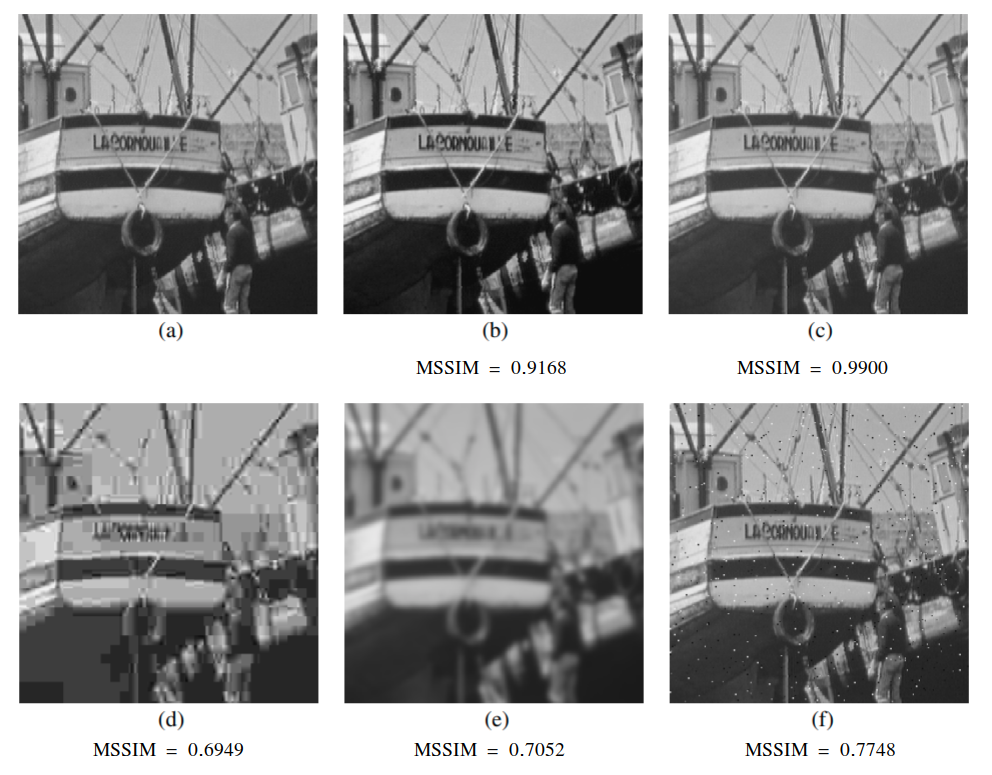
\includegraphics[scale=0.32]{images/mssim_IQA.png}
	\end{center}
	\centering
    \fdireta{wang2004image}
\end{figure}

According to \citeonline{tang2019feature}, the IQA methods are distributed between the subjective assessment and objective assessment categories. The former is based on a well-defined test environment for random observers to label images and provide the final \sigla{MOS}{Mean Opinion Scores}, while the latter is based on the use of strategies such as statistical modeling, machine learning, spatial or spectral image features and so on. It is evident that subjective IQA is demanding; consequently, objective methods are preferred to conduct IQA.

IQA methods are also present within microscopy and its close interaction with image processing. The image acquisition in microscopy techniques may involve lasers, transmitted or reflected light, measurements of atomic force responses, the fluorescence of chemical compounds and several other means. Each technique has an inherent kind of degradation that affects the acquired images or spectra, e.g. the Raman confocal microspectroscopy suffers from the interference of cosmic rays, which yields unexpected peaks in the spectrum.